\section{Kompiuteriniai žaidimai ir vokseliai}

Realaus laiko kompiuterinės grafikos beveik visos inovacijos ir novatoriškos
idėjos atkeliauja per kompiuterinių žaidimų industriją. Ne išimtis ir
vokselizavimo idėja. Čia pateikiama trumpa ir nepilna kompiuterinių žaidimų
istorija, išskirtinį dėmesį rodant vokselizavimo idėjas panaudojusiems
žaidimams.

\subsection{Istorija}

\begin{list}
{
}
{
  \setlength\leftmargin{2.43cm}
  \setlength\labelwidth{3cm}
  \setlength\labelsep{1cm}
}

\item[1986 m.] {\bf Starglider} (Pav. \ref{fig:game_starglider}). Labai
primityvūs trimatę grafiką imituojantys tinkleliai.

\begin{figure}[!ht]
\centering
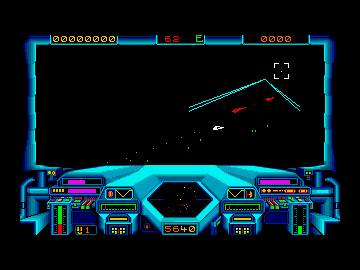
\includegraphics[height=5.0cm]{game_starglider.png}
\caption{Starglider. \emph{MobyGames}\copyright}
\label{fig:game_starglider}
\end{figure}

\item[1988 m.] {\bf F-19 Stealth Fighter}. Tinklelio paviršius užpildomas apvalkalu
ir taip pristatomi poligonai.

\item[1992 m.] {\bf Wolfenstein}. Pristatomos tekstūros. Dėl greičio
atsisakoma tikrojo 3D ir jam imituoti panaudojama spindulių skleidimo
(\emph{Ray Casting}) technologija.

\item[1993 m.] {\bf Comanche} (Pav. \ref{fig:game_comanche}). Panaudojami
vokseliai. Žaidimas pasižymi tiems lai-kams ypač detale aplinka.

\begin{figure}[!ht]
\centering
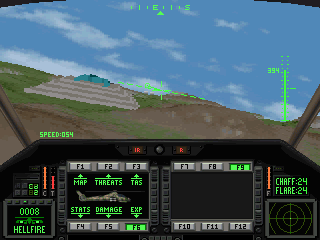
\includegraphics[height=5.0cm]{game_comanche.png}
\caption{Comanche. \emph{NovaLogic}\copyright}
\label{fig:game_comanche}
\end{figure}

\item[1993 m.] {\bf Strike Commander}. Žaidimas, sujungęs tekstūras su
poligonais. Marges-nė ir netokia kampuota kaip Comanche išvaizda, bet iki
pastarojo detalumo lygmens Strike Commander buvo toloka.

\item[1996 m.] {\bf Quake} (Pav. \ref{fig:game_quake}). Prie poligonų ir
tekstūrų pridedami šviesos žemėlapiai (\emph{lightmaps}). Tai leido pasiekti
tuo metu įspūdinga detalumo lygmenį.

\begin{figure}[!ht]
\centering
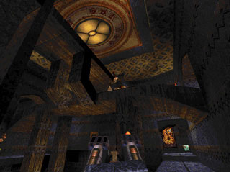
\includegraphics[height=5.0cm]{game_quake.png}
\caption{Quake. \emph{id Software}\copyright}
\label{fig:game_quake}
\end{figure}

\item[1997 m.] {\bf Quake II}. Kompiuterinėje įrangoje įsitvirtina trimatės
grafikos spartintuvai, skirti poligonų vaizdavimui. Šis žaidimas tuo metu bene
geriausiai demonstravo tų įrenginių savybes.

\item[1998 m.] {\bf Delta Force} (Pav. \ref{fig:game_deltaforce}). Ypač
didelėms atviroms aplinkoms buvo panaudotos vokselių technologijos. Žaidimo
variklis buvo pajėgus demonstruoti „begalinius“ atstumus, „begaliniu“
apžvalgos kampu, tačiau vokseliais paremtos technologijos neišnaudojo grafikos
spartintuvų.

\begin{figure}[!ht]
\centering
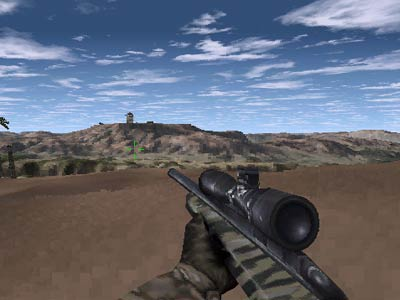
\includegraphics[height=5.0cm]{game_deltaforce.png}
\caption{Delta Force. \emph{NovaLogic}\copyright}
\label{fig:game_deltaforce}
\end{figure}

\item[1999 m.] {\bf Outcast} (Pav. \ref{fig:game_outcast}). Paskutinis, prieš
pertrauką, nusisekęs trimatis žaidimas, naudojęs vokselius.

\begin{figure}[!ht]
\centering
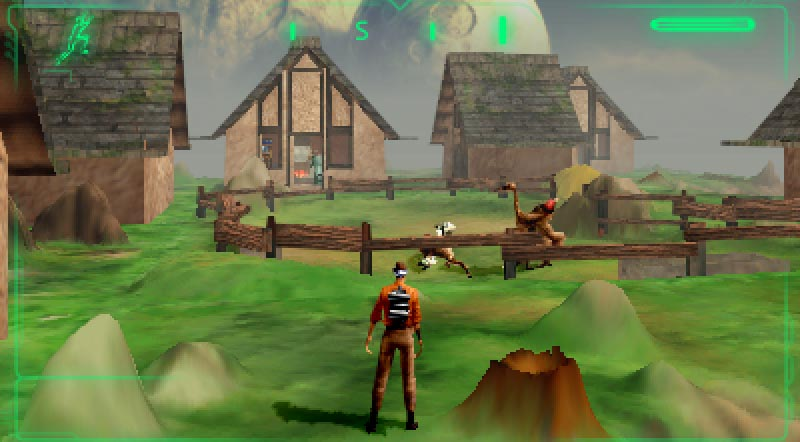
\includegraphics[height=5.0cm]{game_outcast.png}
\caption{Outcast. \emph{Appeal}\copyright}
\label{fig:game_outcast}
\end{figure}

\item[...] Daug, daug tik poligonus naudojančių žaidimų ir žaidimų varikliukų.

\item[2008 m.] \emph{Id Software} Siggraph konferencijoje pristatė vokselių
vizualizavimo technologiją, kuri, tikėtina, bus panaudota būsimajame \emph{Id
Tech 6} varikliuke.

\item[2009 m.] \emph{CryTek} CEDEC konferencijoje paskelbė, kad jų būsimas
varikliukas \emph{Cry-Engine 3} turės galimybę vizualizuoti vokselius.


\end{list}

\subsection{Komentaras}

Visa ši chronologinė tvarka parodo, kad vokseliai kokį dešimtmetį buvo
nenaudojami žaidimų industrijoje. Realaus laiko kompiuterinės grafikos aušroje
buvo bandomos įvairios technologijos ir įvairūs vaizdų generavimo būdai.
Tačiau galiausiai buvo nusistovėta ties poligoniniu vaizdavimo modeliu.

Pagrindinis lūžis įvyko 1996 m. $\sim$ 1997 m. Būtent tada paaiškėjo, kad
trimatės grafikos spartintuvai niekur nedings ir taps neatsiejama asmeninių
kompiuterių ir žaidimų konsolių dalimi.

Vaizdo plokščių atsiradimas stipriai pastūmėjo tiek realaus laiko, tiek visos
kompiuterinės grafi-kos vystymąsi. Tačiau tuo pačiu jų atsiradimas nubrėžė gana
aiškias ribas. Pirmųjų spartintuvų funkcionalumas apsiribojo ties gebėjimu
atvaizduoti daug („daug“ kito nuo laikmečio) trikampių. Taigi, poligoniniai
(trianguliuoti) paviršiai įgijo gana didelį aparatūrinį pranašumą prieš visas
kitas technologijas.

Tačiau viskas vystosi ir keičiasi. Dabartiniai GPU (\emph{Graphics Processing
Unit}) sugeba daugiau nei vien vaizduoti trikampius. Vaizdo plokštės,
nepaisant pavadinimo, patapo bendrinės paskirties, didelį kiekį
mikroprocesorių turinčiais įrenginiais, kurių veikseną galima keisti, nes GPU
be visa ko dar patapo programuojamais -- dabartiniai įrenginiai leidžia
dinamiškai keisti jų pačių veikseną.

Tuo pačiu prasiplėtė ir vaizdavimo ribos, taip atverdamos kelią naujų
vizualizavimo būdų atsiradimui ir senųjų (kartu su vokseliais) grįžimui.
Programuojamos sąsajos leidžia kūrėjams stipriai pakeisti GPU veikseną taip,
kad anos sugeba greitai ir gerai vizualizuoti net tik poligonus.

